\documentclass[10pt]{beamer}
\usepackage[utf8]{inputenc}
\usetheme{Berlin}
\usefonttheme{professionalfonts}
\usecolortheme{orchid}

\usepackage{blindtext}
\usepackage{amsmath}

\usepackage{array}       
\usepackage{tabularx}
\usepackage{dcolumn} 
  \newcolumntype{d}[1]{D{.}{.}{#1}}    
\usepackage{booktabs}

\usepackage{tikz}
\usepackage{pgfplots}
\pgfplotsset{compat=1.17}
\usepgfplotslibrary{colorbrewer}
\usepackage{collcell}

 %The min, mid and max values
\newcommand*{\MinNumber}{0.0}%
\newcommand*{\MidNumber}{0.5} %
\newcommand*{\MaxNumber}{1.0}%

%Apply the gradient macro
\newcommand{\ApplyGradient}[1]{%
        \ifdim #1 pt > \MidNumber pt
            \pgfmathsetmacro{\PercentColor}{max(min(100.0*(#1 - \MidNumber)/(\MaxNumber-\MidNumber),100.0),0.00)} %
            \hspace{-0.33em}\colorbox{purple!\PercentColor!yellow}{#1}
        \else
            \pgfmathsetmacro{\PercentColor}{max(min(100.0*(\MidNumber - #1)/(\MidNumber-\MinNumber),100.0),0.00)} %
            \hspace{-0.33em}\colorbox{red!\PercentColor!yellow}{#1}
        \fi
}

\newcolumntype{R}{>{\collectcell\ApplyGradient}c<{\endcollectcell}}
\renewcommand{\arraystretch}{0}
\setlength{\fboxsep}{3mm} % box size
\setlength{\tabcolsep}{0pt}


\title{Digital Tools for Finance}
\subtitle{If a tree fell in your random forest, would anyone notice?}
\author{Maximilian Weber \and David Jaggi}
\institute{University of Zurich}
\date{December 2021}

\begin{document}
% ---------------------------------------------------------------------------
\frame{\titlepage}
% ---------------------------------------------------------------------------
\begin{frame}{Table of Contents}
    \framesubtitle{Table of Contents}
    \tableofcontents
\end{frame}
% ---------------------------------------------------------------------------
\section{Figures}
\begin{frame}{Frame 1}
    \framesubtitle{Subtitle 1}
    \begin{figure}
    \centering
        \begin{minipage}{.45\textwidth}
          \centering
          \includegraphics[width=.75\linewidth]{example-image-a}
          \caption{Very nice image A.}
          \label{fig:test-a}
        \end{minipage}%
        \begin{minipage}{.45\textwidth}
          \centering
          \includegraphics[width=.75\linewidth]{example-image-b}
          \caption{Also nice image B.}
          \label{fig:test-b}
        \end{minipage}
    \end{figure}
\end{frame}
% ---------------------------------------------------------------------------
\section{Theorem}
\begin{frame}{Frame 2}
    \framesubtitle{Subtitle 2}
    \begin{theorem}{Example Theorem}
        Let \(f\) be a function whose derivative exists in every point, then \(f\) 
        is a continuous function.
    \end{theorem}
\end{frame}
% ---------------------------------------------------------------------------
\section{Gather}
\begin{frame}{Frame 3}
    \framesubtitle{Subtitle 3}
        \begin{gather}
            1+1=2 \\
            2+2=4
        \end{gather}
\end{frame}
% ---------------------------------------------------------------------------
\section{DColumn}
\begin{frame}{Frame 4}
    \framesubtitle{Subtitle 4}
        % table using D from dcolumn package
    \begin{table}   
  \centering
  \caption{Table with package dcolumn}
  \begin{tabularx}{\textwidth}{l*{3}{d{-2}}}
  \toprule
            &  \multicolumn{1}{X}{\centering col A} &
\multicolumn{1}{X}{\centering col B} &
\multicolumn{1}{X}{\centering col C} \\
\cmidrule(lr){2-2} \cmidrule(lr){3-3} \cmidrule(lr){4-4}
  \midrule  
       North &      2'228.0   &   0.3 &  10.6 \\    
       South &        689.2 &   0.8   &   2.6 \\
  \bottomrule
  \end{tabularx}     
\end{table}
\end{frame}
% ---------------------------------------------------------------------------
\section{Heatmap}
\begin{frame}{Frame 5}
    \begin{table}
        \begin{center}
        \caption{Correlation table}
            \begin{tabular}{*{5}{R}}
              1.00 & 0.50 & 0.30 & 0.12 & 0.29 \\
              0.50 & 1.00 & 0.49 & 0.18 & 0.95 \\
              0.30 & 0.49 & 1.00 & 0.40 & 0.20 \\
              0.12 & 0.18 & 0.40 & 1.00 & 0.62 \\
              0.29 & 0.95 & 0.20 & 0.62 & 1.00 \\
            \end{tabular}
        \end{center}
    \end{table}
\end{frame}
% ---------------------------------------------------------------------------
\section{Plot}
\begin{frame}{Frame 6}
    \begin{figure}
        \caption{Line plot using colorbrewer}
        \centering
        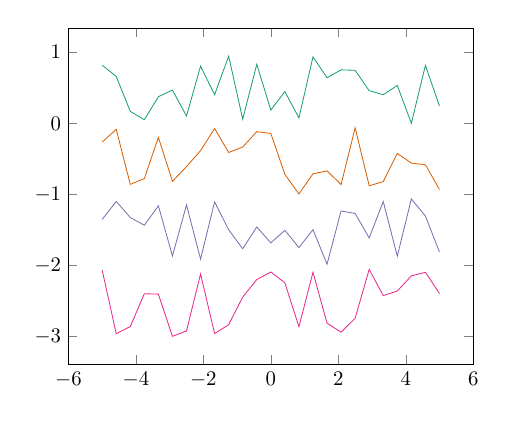
\begin{tikzpicture}[scale=0.75]
        \begin{axis}[cycle list/Dark2]
            \addplot {rnd};
            \addplot {rnd-1};
            \addplot {rnd-2};
            \addplot {rnd-3};
            \end{axis}
        \end{tikzpicture}
    \end{figure}
\end{frame}
% ---------------------------------------------------------------------------

\end{document}